\begin{frame}
	\frametitle{Biased Clump Properties}
	\begin{center}
		\begin{tabular}{c c}
			initial set-up 	& clumps found by \phew\ \\[.5em]
			%
			%	 
			{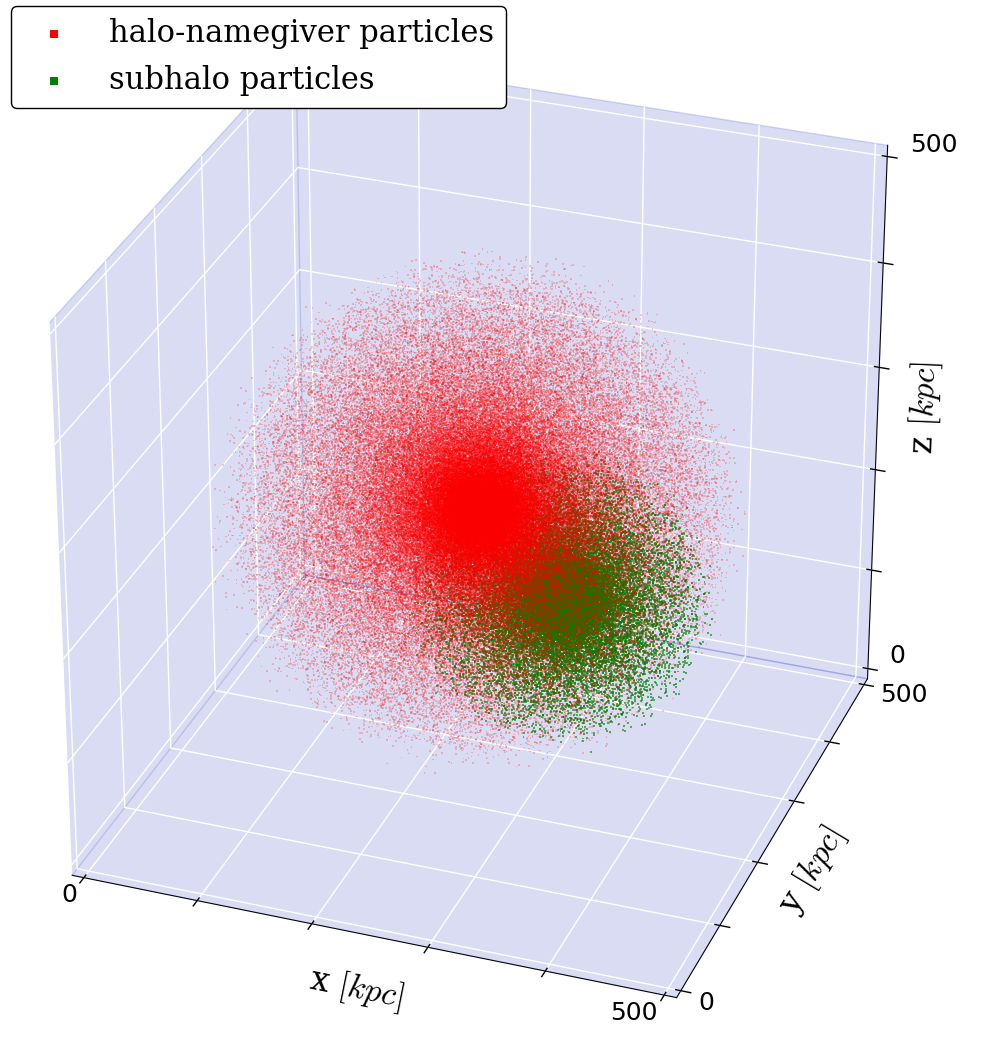
\includegraphics[width = .4\textwidth]{../report/images/dice-two/dice-two-original-plot.png}} \hspace*{-1em} 	& 
			{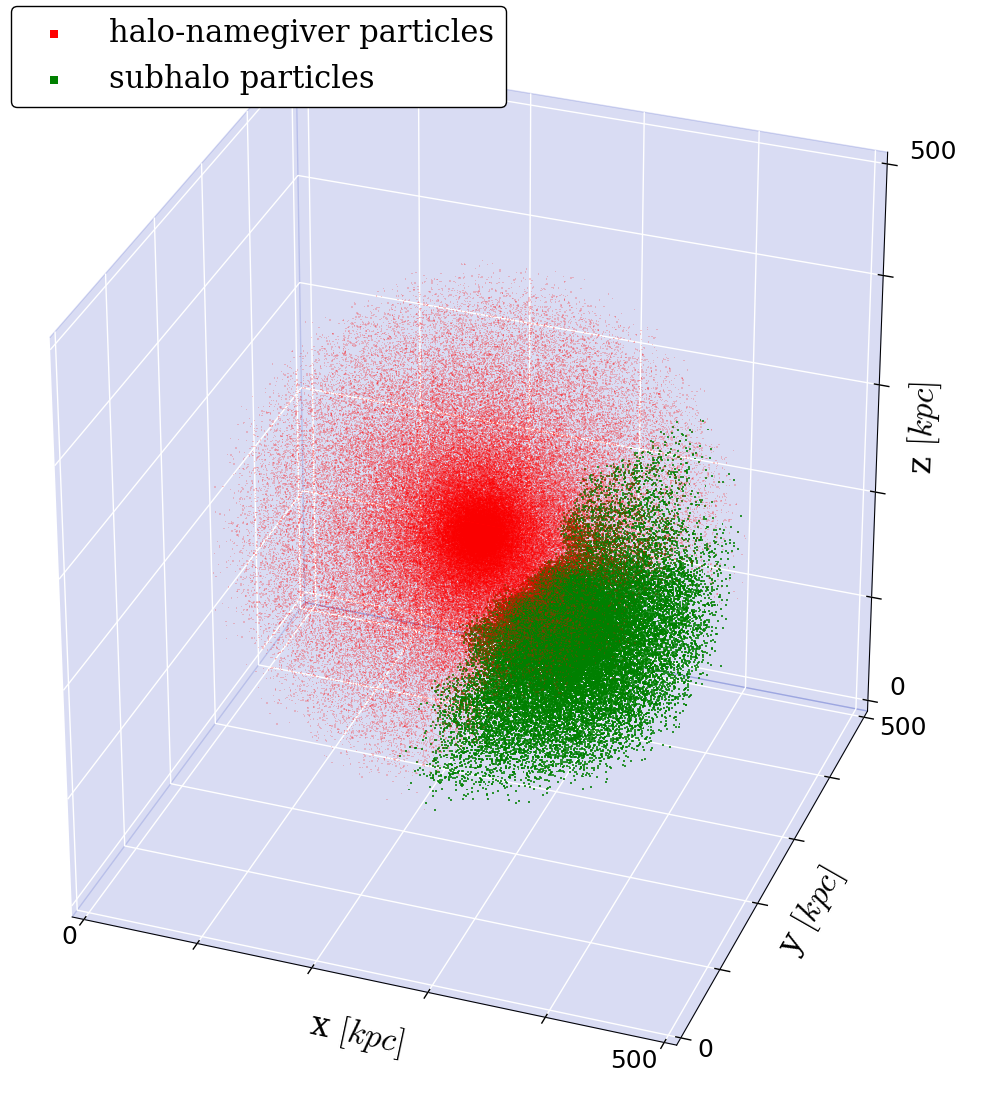
\includegraphics[width = .4\textwidth]{../report/images/dice-two/dice-two-plot-halo1451-phew.png}}
		\end{tabular}
	\end{center}

	The identified clump properties will be biased:
	\begin{itemize}
		\item Missing particles: Subhalo is cut off
		\item Alien particles: Subhalo in contaminated by host's particles
	\end{itemize}
\end{frame}



\begin{frame}
	\frametitle{Biased Clump Properties}
	
	It seems likely that the clump properties after particle unbinding should be closer to the known ones, particularly so if only exclusively bound particles are considered.\\[1em]
	
	$\Rightarrow$  recompute the clump properties after unbinding and use this updated information to go through the entire procedure again.
	
	Reiterate until the bulk velocity of each clump converges:
	\begin{equation*}
	\text{bulk velocity converged} \Leftrightarrow \left | \frac{v_{bulk,old} - v_{bulk,new}}{v_{bulk,old}} \right | < \varepsilon
	\end{equation*}
	where $\varepsilon$ is a user-defined convergence limit.
\end{frame}


\begin{frame}
	\frametitle{Results: Converging of the bulk velocity for the \dt-dataset}
	
The deviation $D_{orig} = \left | 	 \frac{v_{bulk} - v_{orig}}{v_{orig}}				\right |$  from the originally set bulk velocity to the computed bulk velocity for the subhalo of the \dt-dataset in dependence of the convergence limit $\varepsilon$:

	
	\begin{table}[!htb]
		\begin{centering}
			\begin{tabular}[t]{r | l | r | l }
				$\varepsilon$     &  \texttt{niter}  		&	$D_{orig}$	\\
				\hline
				0.5       &    	 		2    	&	0.2326  \\
				0.1       &   	       	4    	&	0.0419	\\
				0.01      &           	7    	&	0.0024	\\
				0.001     &            	8    	&	0.0014  \\       
				0.0001    &        		10    	&	0.0009 	\\
			\end{tabular}
		\end{centering}
	\end{table}
	
	The bulk velocity computation needed \texttt{niter} iterations to converge.
	
\end{frame}




\begin{frame}
	\frametitle{Results: \dt-dataset}
	
	\begin{tabular}{c c}
		\neigh\ 	& \iter \\[1.5em]
		%
		%	 
		{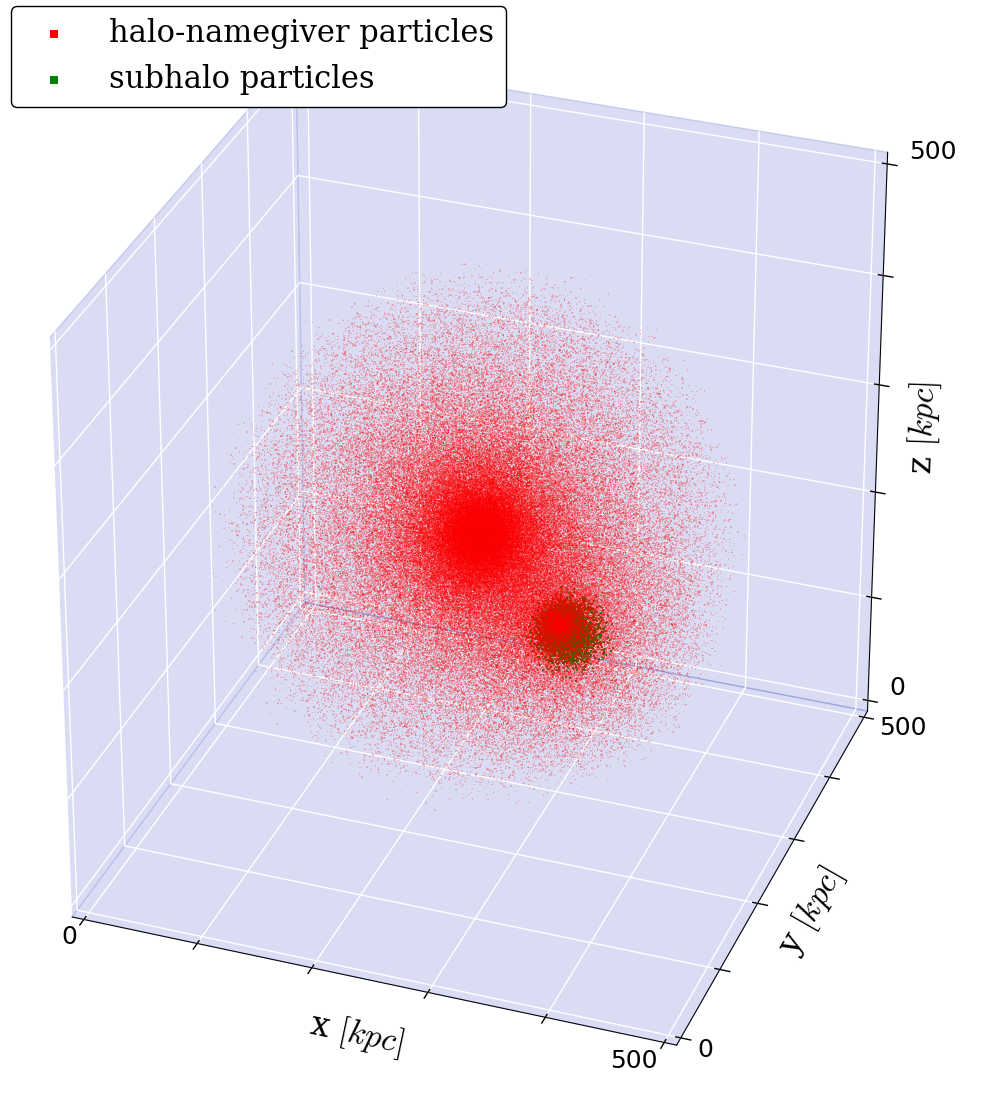
\includegraphics[width = .49\textwidth]{../report/images/dice-two/dice-two-plot-halo1451-saddle.png}} &
		{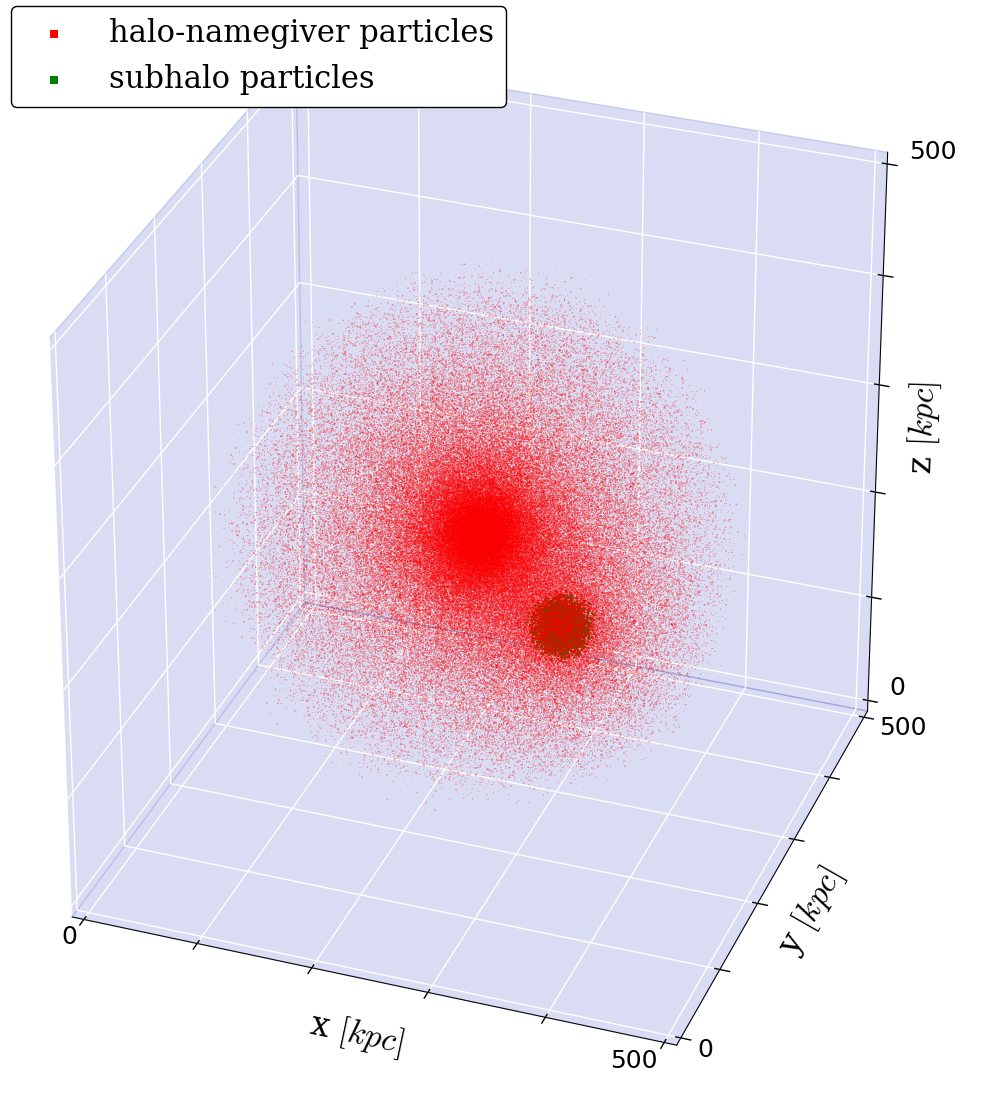
\includegraphics[width = .49\textwidth]{../report/images/dice-two/dice-two-plot-halo1451-iter.png}} \hspace*{-1em} 
	\end{tabular}
\end{frame}





\begin{frame}
	\frametitle{Results: \dt-dataset: halo-namegiver particles only}
	
	\begin{tabular}{c c}
		\neigh\ 	& \iter \\[1.5em]
		%
		%	 
		{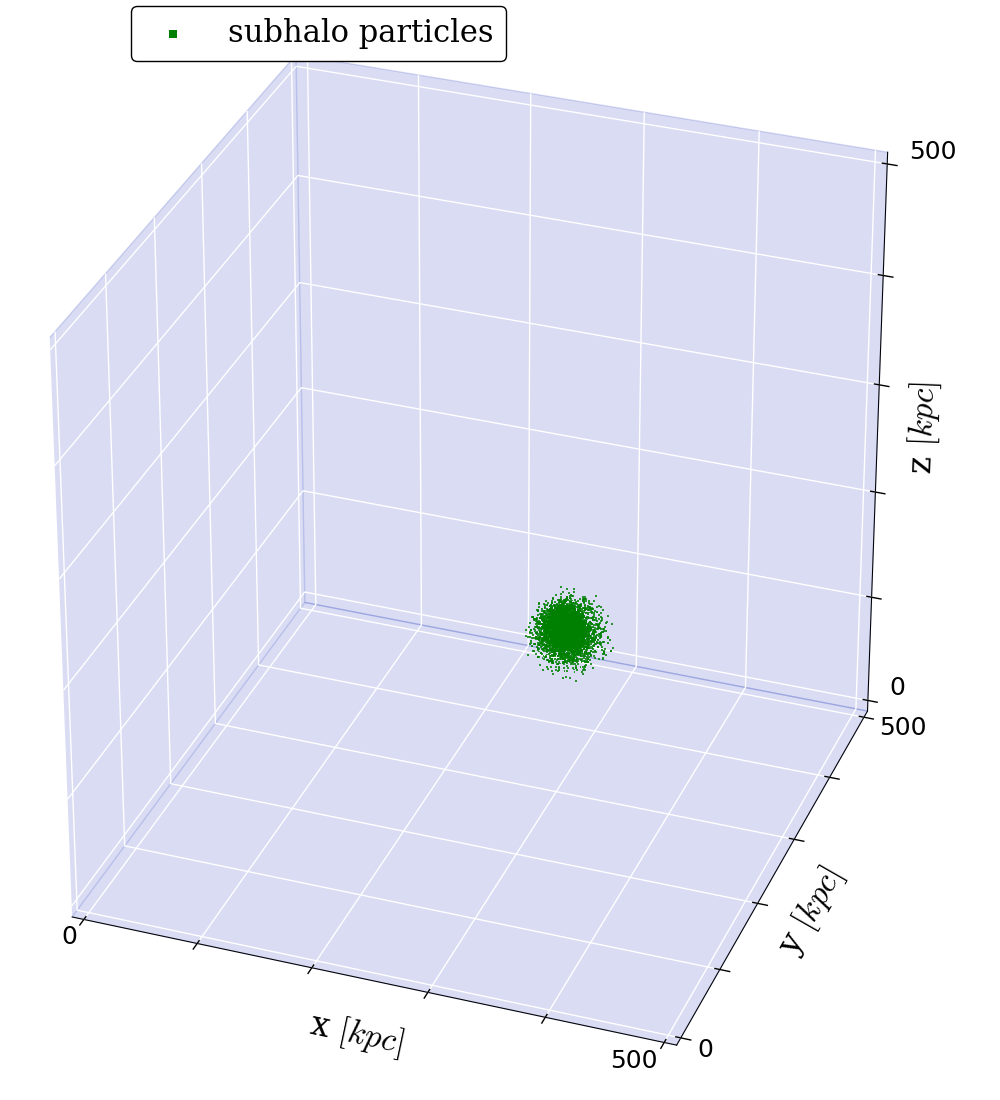
\includegraphics[width = .49\textwidth]{../report/images/dice-two/dice-two-plot-subhalo-saddle.png}}	&
		{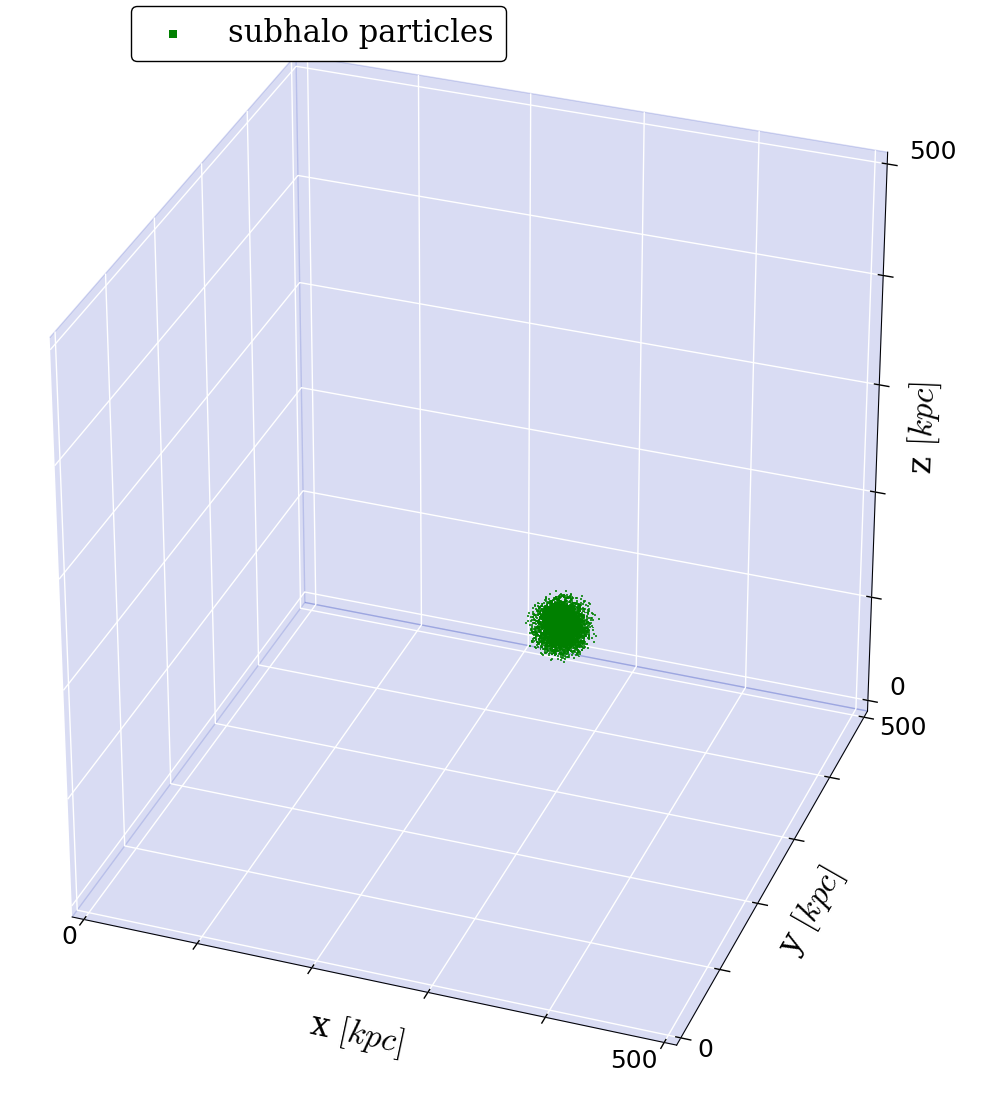
\includegraphics[width = .49\textwidth]{../report/images/dice-two/dice-two-plot-subhalo-iter.png}}  
	\end{tabular}
\end{frame}




%\begin{frame}
%	\frametitle{Results: \ds-dataset}
%	
%	\begin{tabular}{c c}
%		\neigh\ 	& \iter \\[1.5em]
%		%
%		%
%		
%		{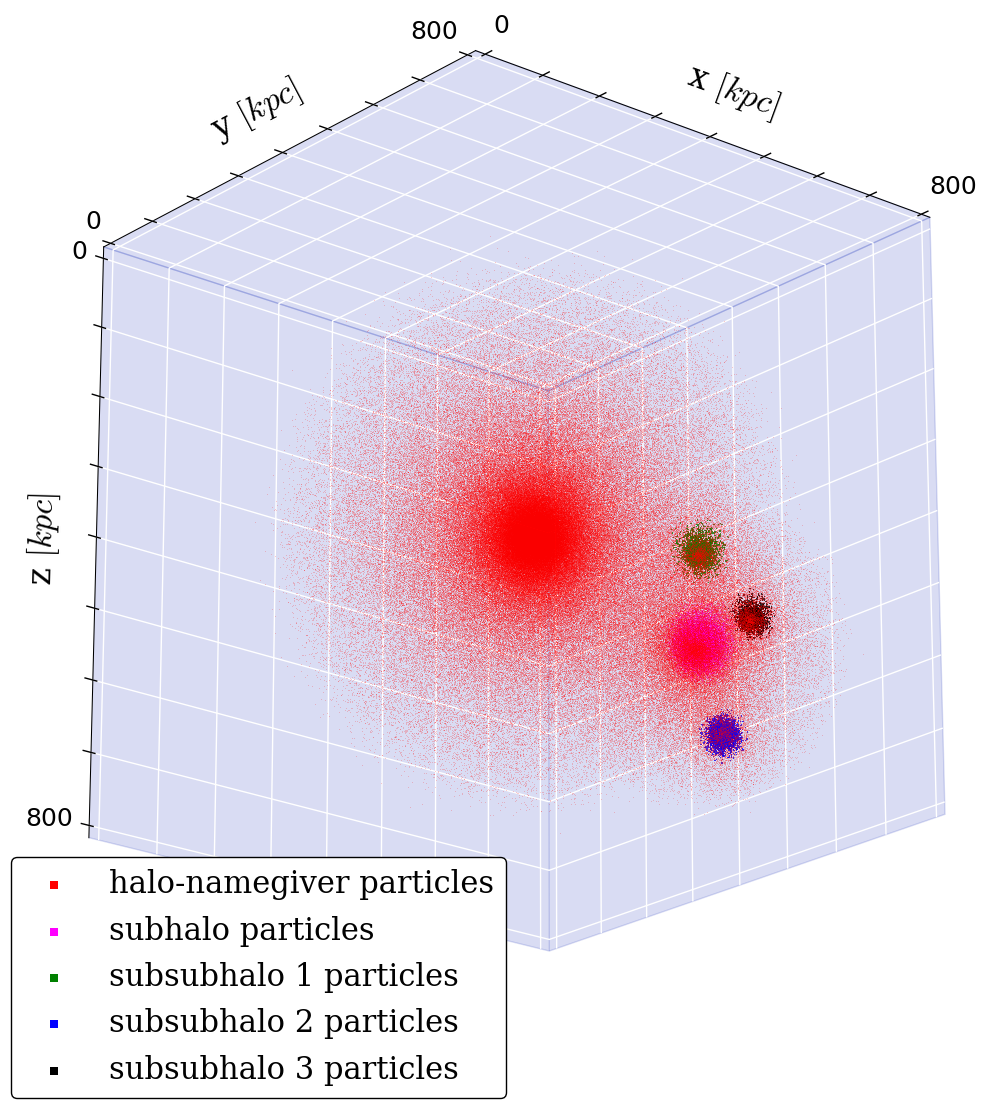
\includegraphics[width = .49\textwidth]{../report/images/dice-sub/dice-sub-plot-halo1-saddle.png}}	&		 
%		{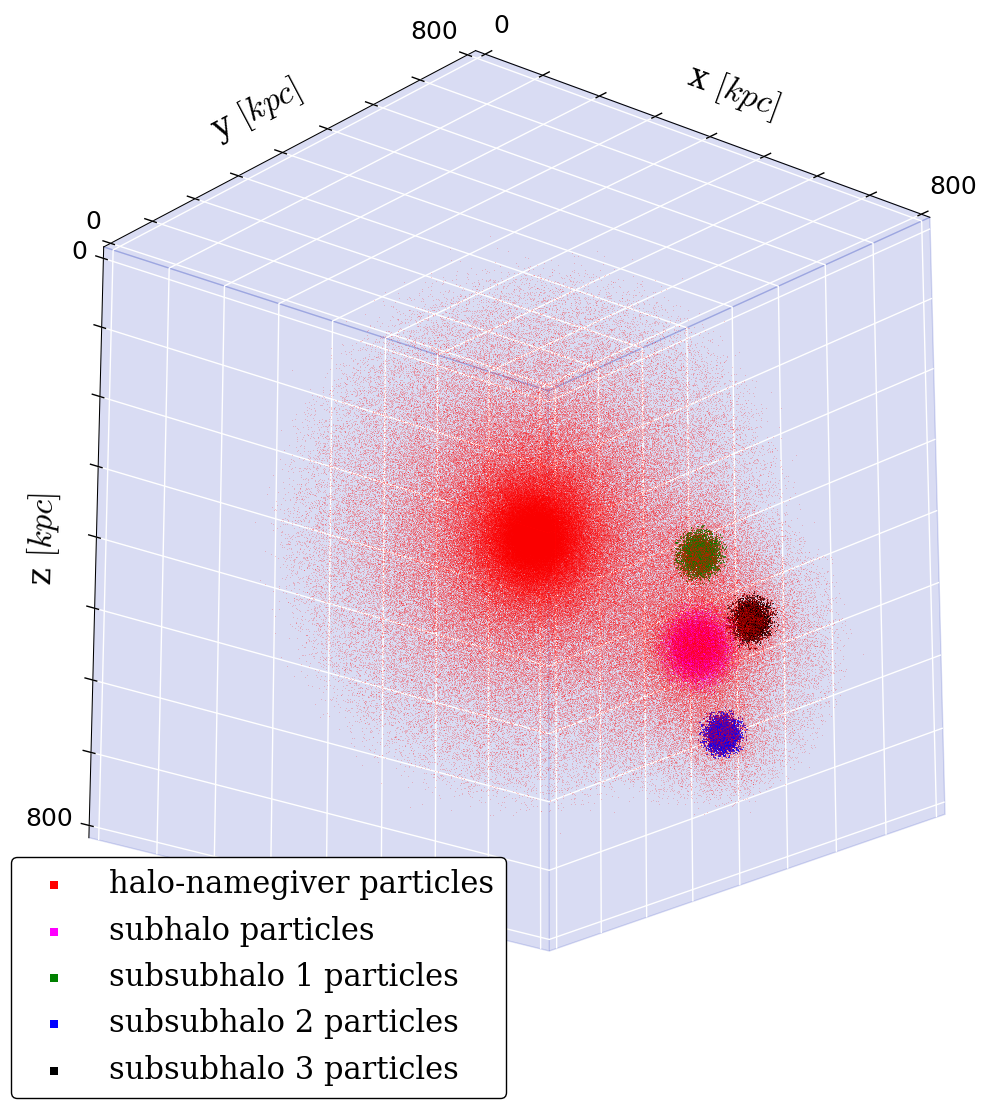
\includegraphics[width = .49\textwidth]{../report/images/dice-sub/dice-sub-plot-halo1-iter.png}} 	
%	\end{tabular}
%\end{frame}
%
%
%
%\begin{frame}
%	\frametitle{Results: \ds-dataset: halo-namegiver particles only}
%	
%	\begin{tabular}{c c}
%		\neigh\ 	& \iter \\[1.5em]
%		%
%		%	 
%		{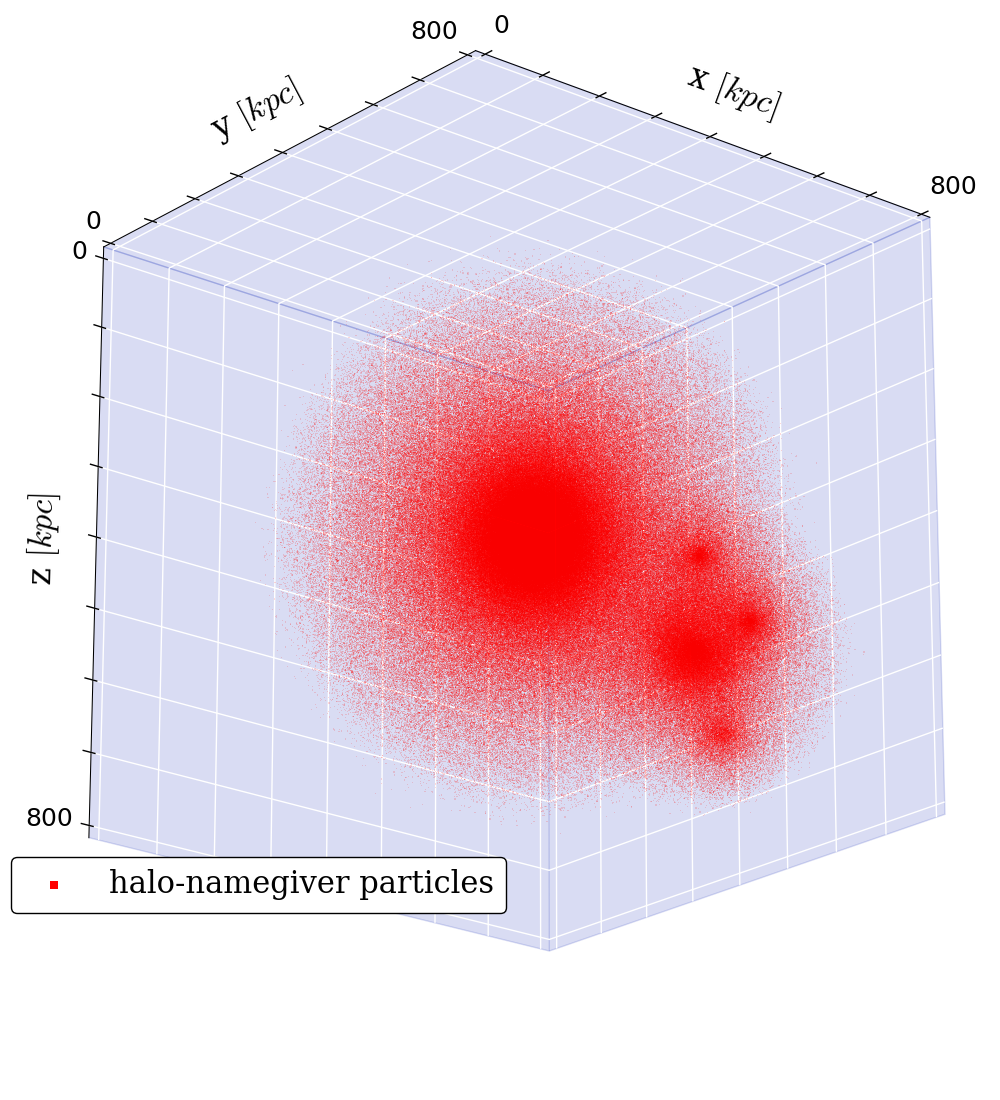
\includegraphics[width = .49\textwidth]{../report/images/dice-sub/dice-sub-halo-only-saddle.png}} \hspace*{-1em} 	& 
%		{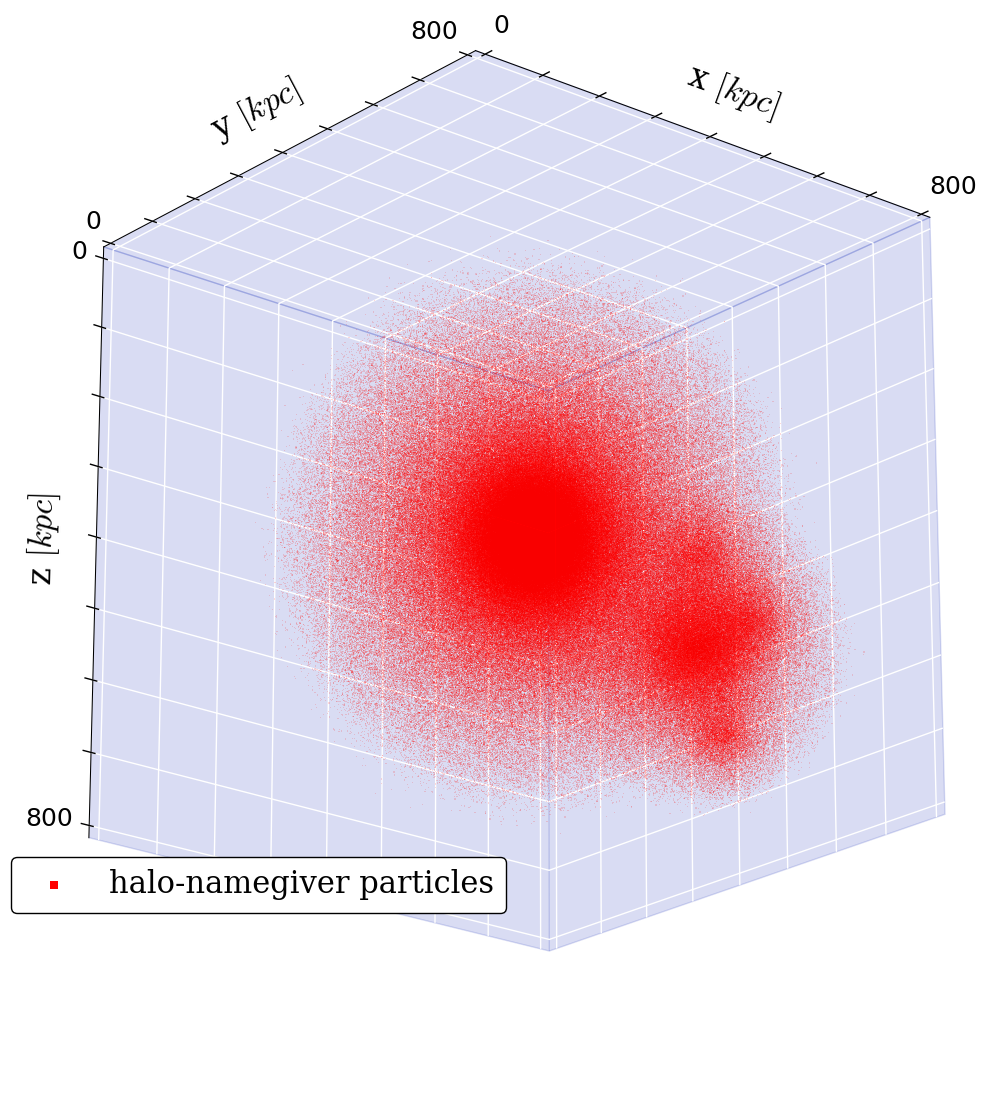
\includegraphics[width = .49\textwidth]{../report/images/dice-sub/dice-sub-halo-only-iter.png}}
%	\end{tabular}
%\end{frame}



\begin{frame}
	\frametitle{Results: \cosmo-dataset: halo-namegiver particles only}
	
	\begin{tabular}{c c}
		\neigh\ 	& \iter \\[1.5em]
		%
		%	 
		{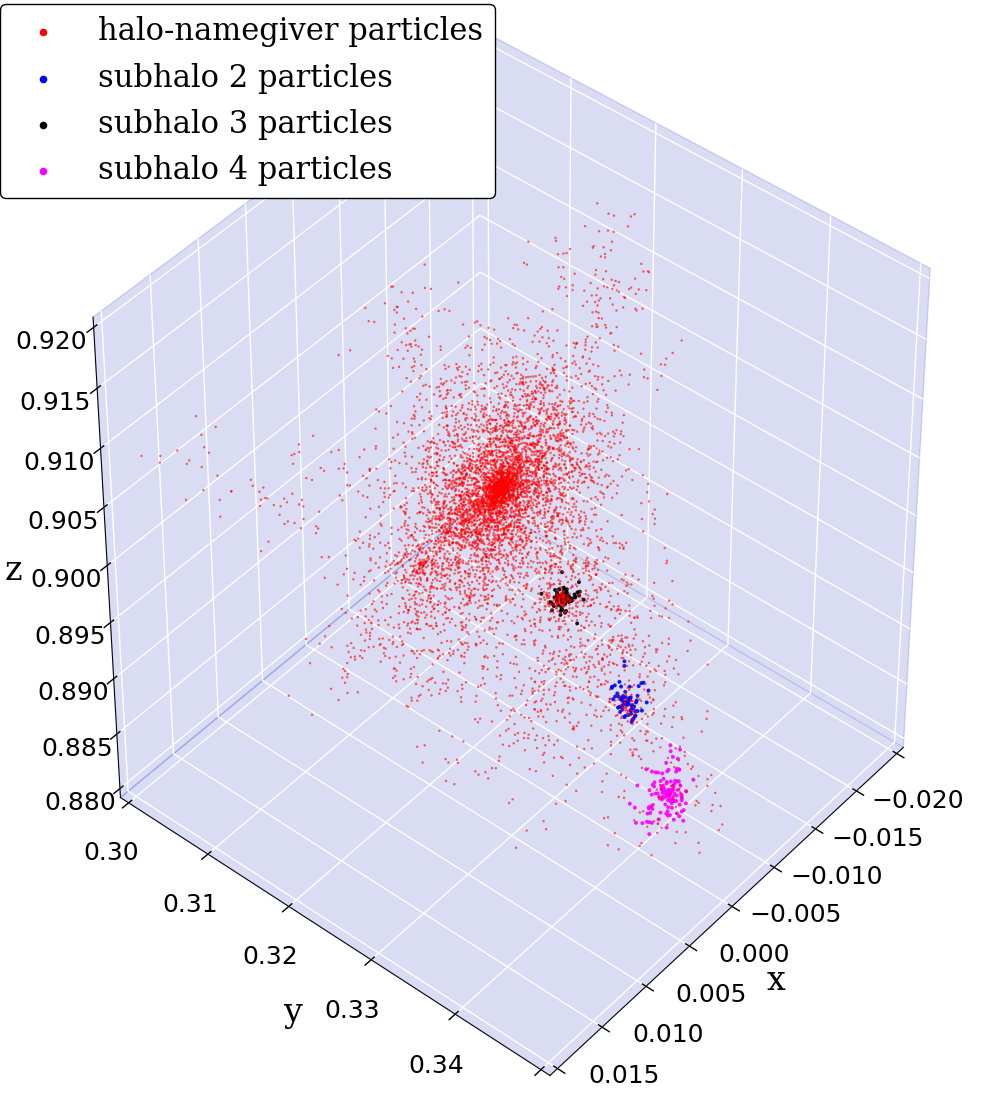
\includegraphics[width = .49\textwidth]{../report/images/cosmo/cos-halo-66858-saddle.png}}	& 
		{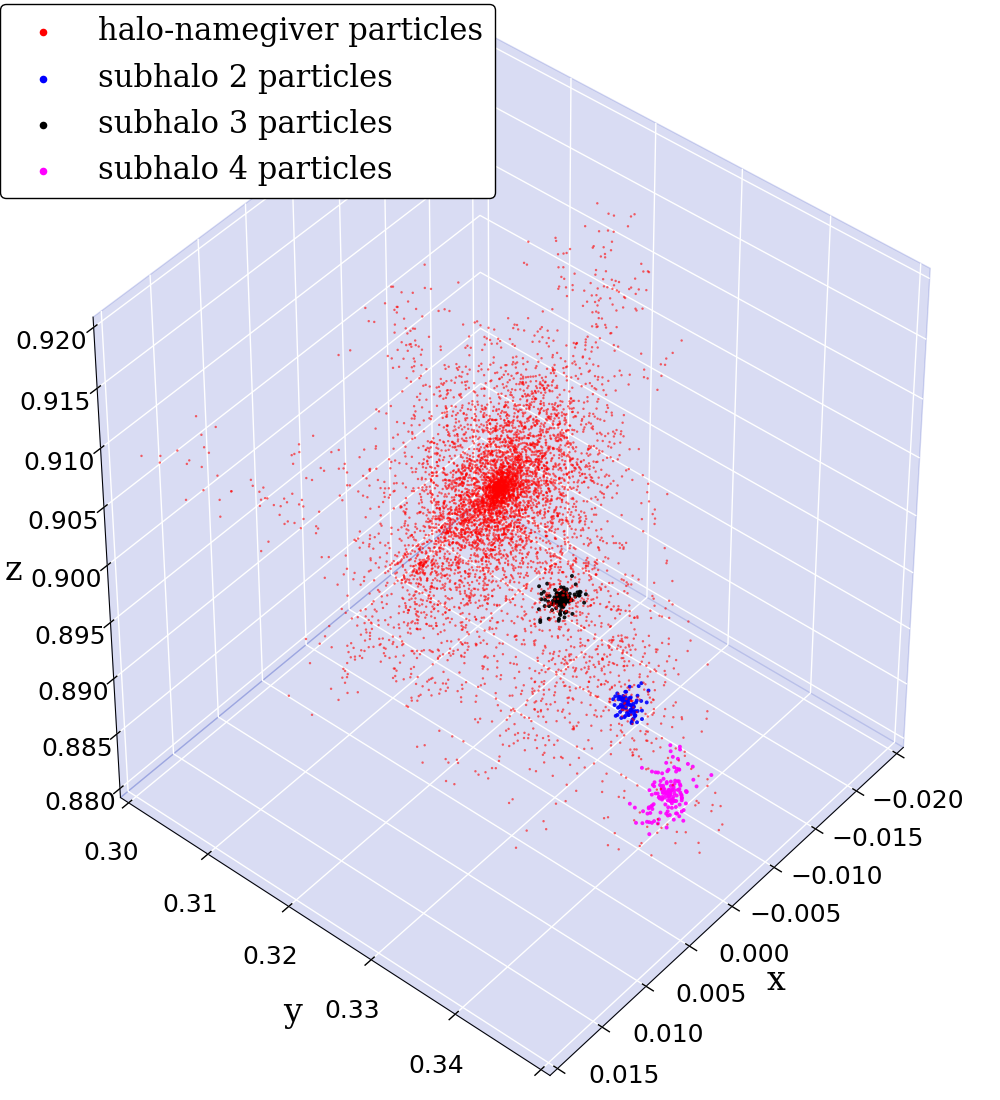
\includegraphics[width = .49\textwidth]{../report/images/cosmo/cos-halo-66858-iter.png}}
	\end{tabular}
\end{frame}



\begin{frame}
	\frametitle{Results: \cosmo-dataset: halo-namegiver particles only}
	
	\begin{tabular}{c c}
		\neigh\ 	& \iter \\[1.5em]
		%
		%	 
		{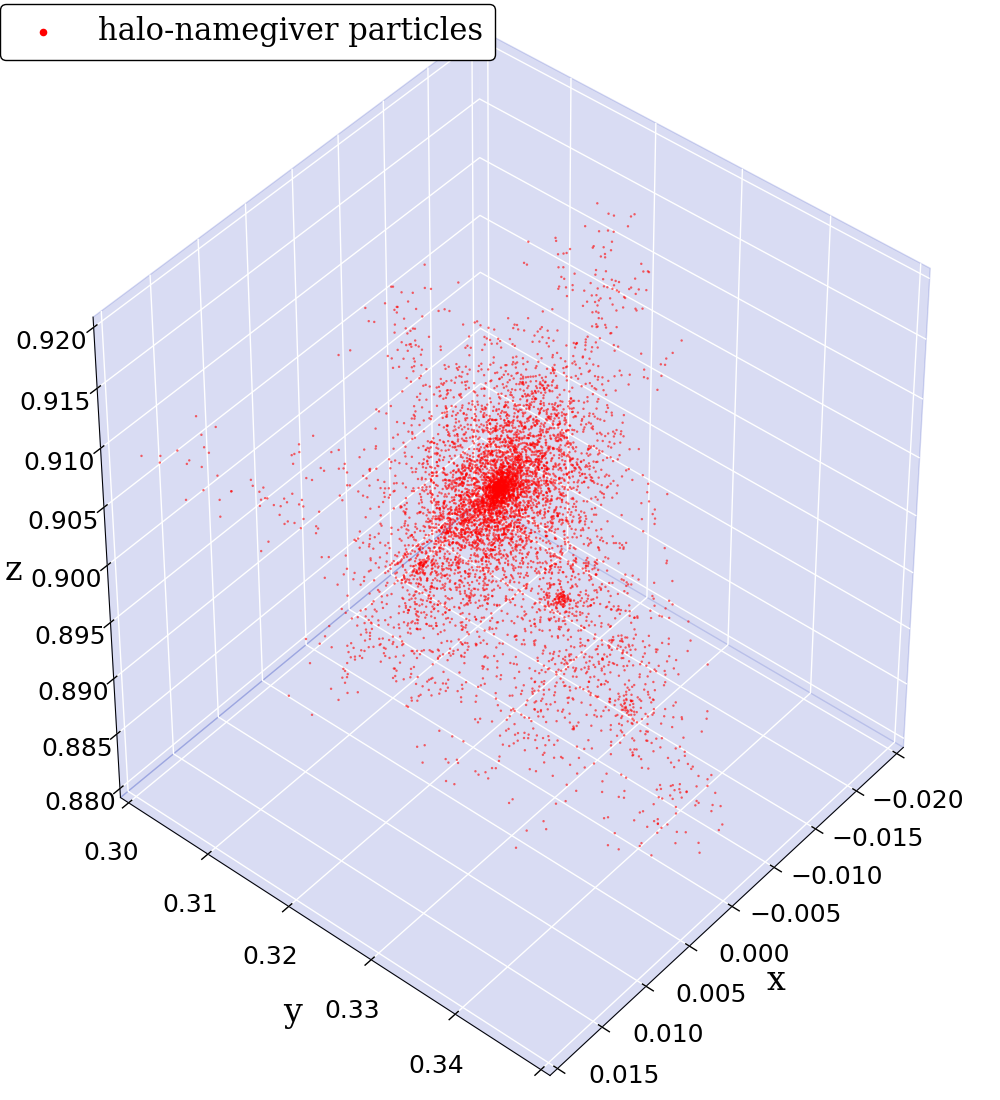
\includegraphics[width = .49\textwidth]{../report/images/cosmo/cos-halo-66858-halo-only-saddle.png}} \hspace*{-1em} 	& 
		{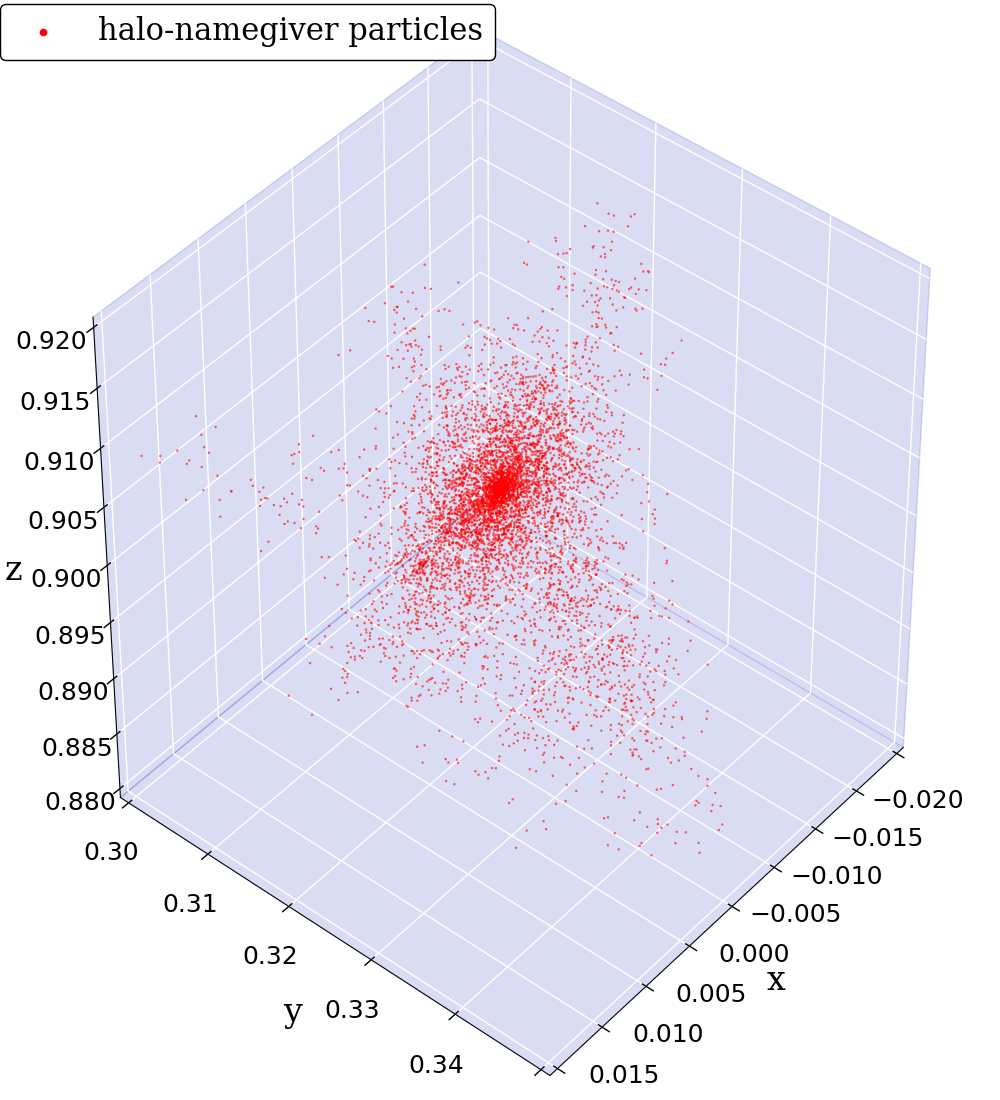
\includegraphics[width = .49\textwidth]{../report/images/cosmo/cos-halo-66858-halo-only-iter.png}}
	\end{tabular}
\end{frame}